\documentclass[11pt]{article}
\usepackage[textwidth=18.0cm, textheight=23.0cm, top=2.0cm]{geometry}
\usepackage{pst-all}
\usepackage{amssymb}
\usepackage{tikz}
\usepackage{underscore}\begin{document}
\pagestyle{empty}


ClassName: \underline{\textbf{Class_07.2bp-20}}
\par
BinSize: \underline{\textbf{100 × 100}}
\par
ReduceSize: \underline{\textbf{100 × 100}}
\par
TypeNum: \underline{\textbf{59}}
\par
Num: \underline{\textbf{60}}
\par
OutS: \underline{\textbf{170000}}
\par
InS: \underline{\textbf{146727}}
\par
Rate: \underline{\textbf{0.863}}
\par
UB: \underline{\textbf{17}}
\par
LB0: \underline{\textbf{17}}
\par
LB: \underline{\textbf{17}}
\par
LBWithCut: \underline{\textbf{17}}
\par
NodeCut: \underline{\textbf{0}}
\par
ExtendedNodeCnt: \underline{\textbf{1}}
\par
GenNodeCnt: \underline{\textbf{1}}
\par
PrimalNode: \underline{\textbf{0}}
\par
ColumnCount: \underline{\textbf{17}}
\par
TotalCutCount: \underline{\textbf{0}}
\par
RootCutCount: \underline{\textbf{0}}
\par
LPSolverCnt: \underline{\textbf{1}}
\par
PricingSolverCnt: \underline{\textbf{0}}
\par
BranchAndBoundNum: \underline{\textbf{1}}
\par
isOpt: \underline{\textbf{true}}
\par
TimeOnInitSolution: \underline{\textbf{600.000 s}}
\par
TimeOnPrimal: \underline{\textbf{0.000 s}}
\par
TimeOnPricing: \underline{\textbf{0.000 s}}
\par
TimeOnRmp: \underline{\textbf{0.078 s}}
\par
TotalTime: \underline{\textbf{600.328 s}}
\par
\newpage


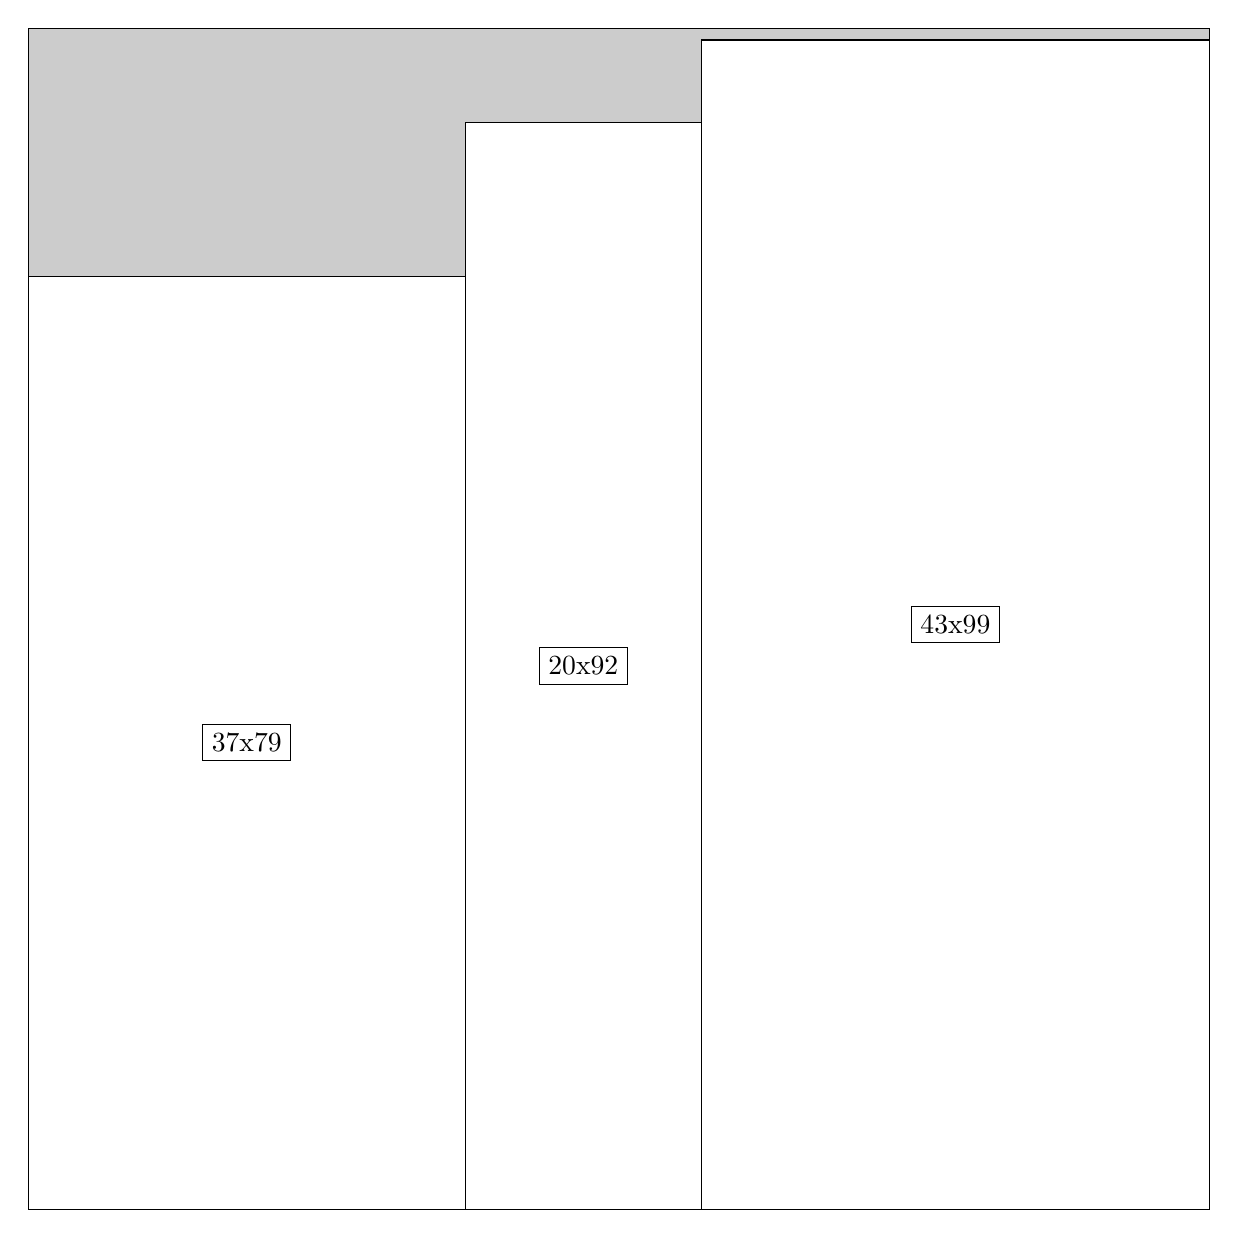
\begin{tikzpicture}[shorten >=1pt,scale=1.0,every node/.style={scale=1.0},->]
\tikzstyle{vertex}=[circle,fill=black!25,minimum size=14pt,inner sep=0pt]
\filldraw[fill=gray!40!white, draw=black] (0,0) rectangle (15.0,15.0);
\foreach \name/\x/\y/\w/\h in {43x99/8.549999999999999/0.0/6.45/14.85,20x92/5.55/0.0/3.0/13.799999999999999,37x79/0.0/0.0/5.55/11.85}
\filldraw[fill=white!40!white, draw=black] (\x,\y) rectangle node[draw] (\name) {\name} ++(\w,\h);
\end{tikzpicture}


w =43 , h =99 , x =57 , y =0 , v =4257
\par
w =20 , h =92 , x =37 , y =0 , v =1840
\par
w =37 , h =79 , x =0 , y =0 , v =2923
\par
\newpage


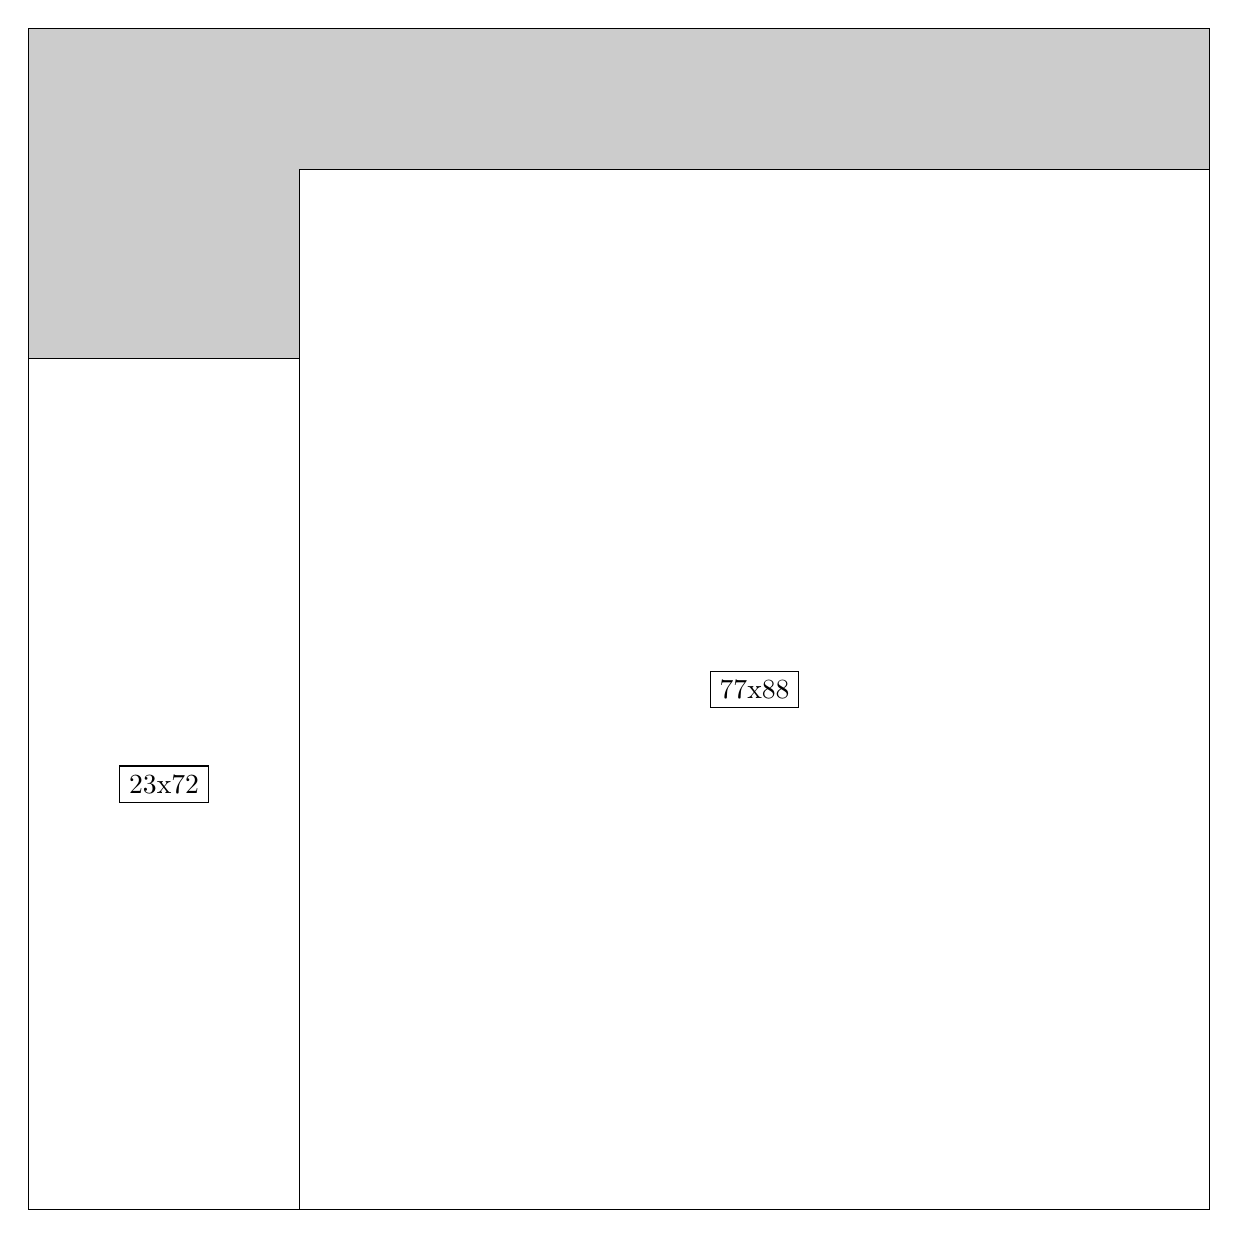
\begin{tikzpicture}[shorten >=1pt,scale=1.0,every node/.style={scale=1.0},->]
\tikzstyle{vertex}=[circle,fill=black!25,minimum size=14pt,inner sep=0pt]
\filldraw[fill=gray!40!white, draw=black] (0,0) rectangle (15.0,15.0);
\foreach \name/\x/\y/\w/\h in {77x88/3.4499999999999997/0.0/11.549999999999999/13.2,23x72/0.0/0.0/3.4499999999999997/10.799999999999999}
\filldraw[fill=white!40!white, draw=black] (\x,\y) rectangle node[draw] (\name) {\name} ++(\w,\h);
\end{tikzpicture}


w =77 , h =88 , x =23 , y =0 , v =6776
\par
w =23 , h =72 , x =0 , y =0 , v =1656
\par
\newpage


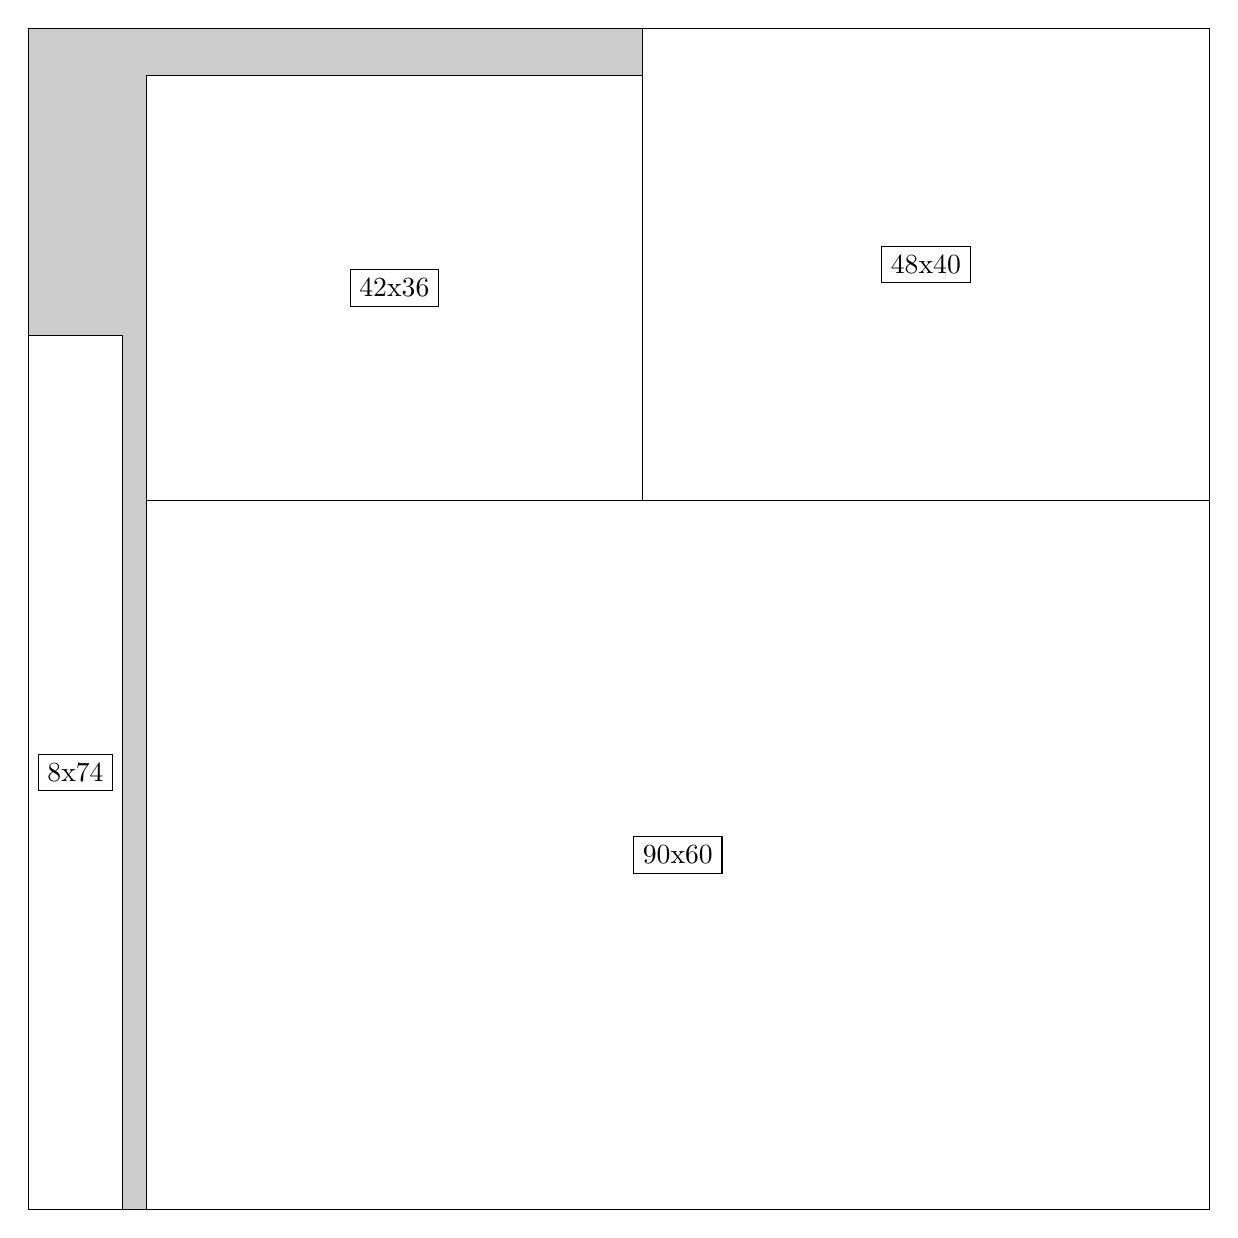
\begin{tikzpicture}[shorten >=1pt,scale=1.0,every node/.style={scale=1.0},->]
\tikzstyle{vertex}=[circle,fill=black!25,minimum size=14pt,inner sep=0pt]
\filldraw[fill=gray!40!white, draw=black] (0,0) rectangle (15.0,15.0);
\foreach \name/\x/\y/\w/\h in {90x60/1.5/0.0/13.5/9.0,48x40/7.8/9.0/7.199999999999999/6.0,42x36/1.5/9.0/6.3/5.3999999999999995,8x74/0.0/0.0/1.2/11.1}
\filldraw[fill=white!40!white, draw=black] (\x,\y) rectangle node[draw] (\name) {\name} ++(\w,\h);
\end{tikzpicture}


w =90 , h =60 , x =10 , y =0 , v =5400
\par
w =48 , h =40 , x =52 , y =60 , v =1920
\par
w =42 , h =36 , x =10 , y =60 , v =1512
\par
w =8 , h =74 , x =0 , y =0 , v =592
\par
\newpage


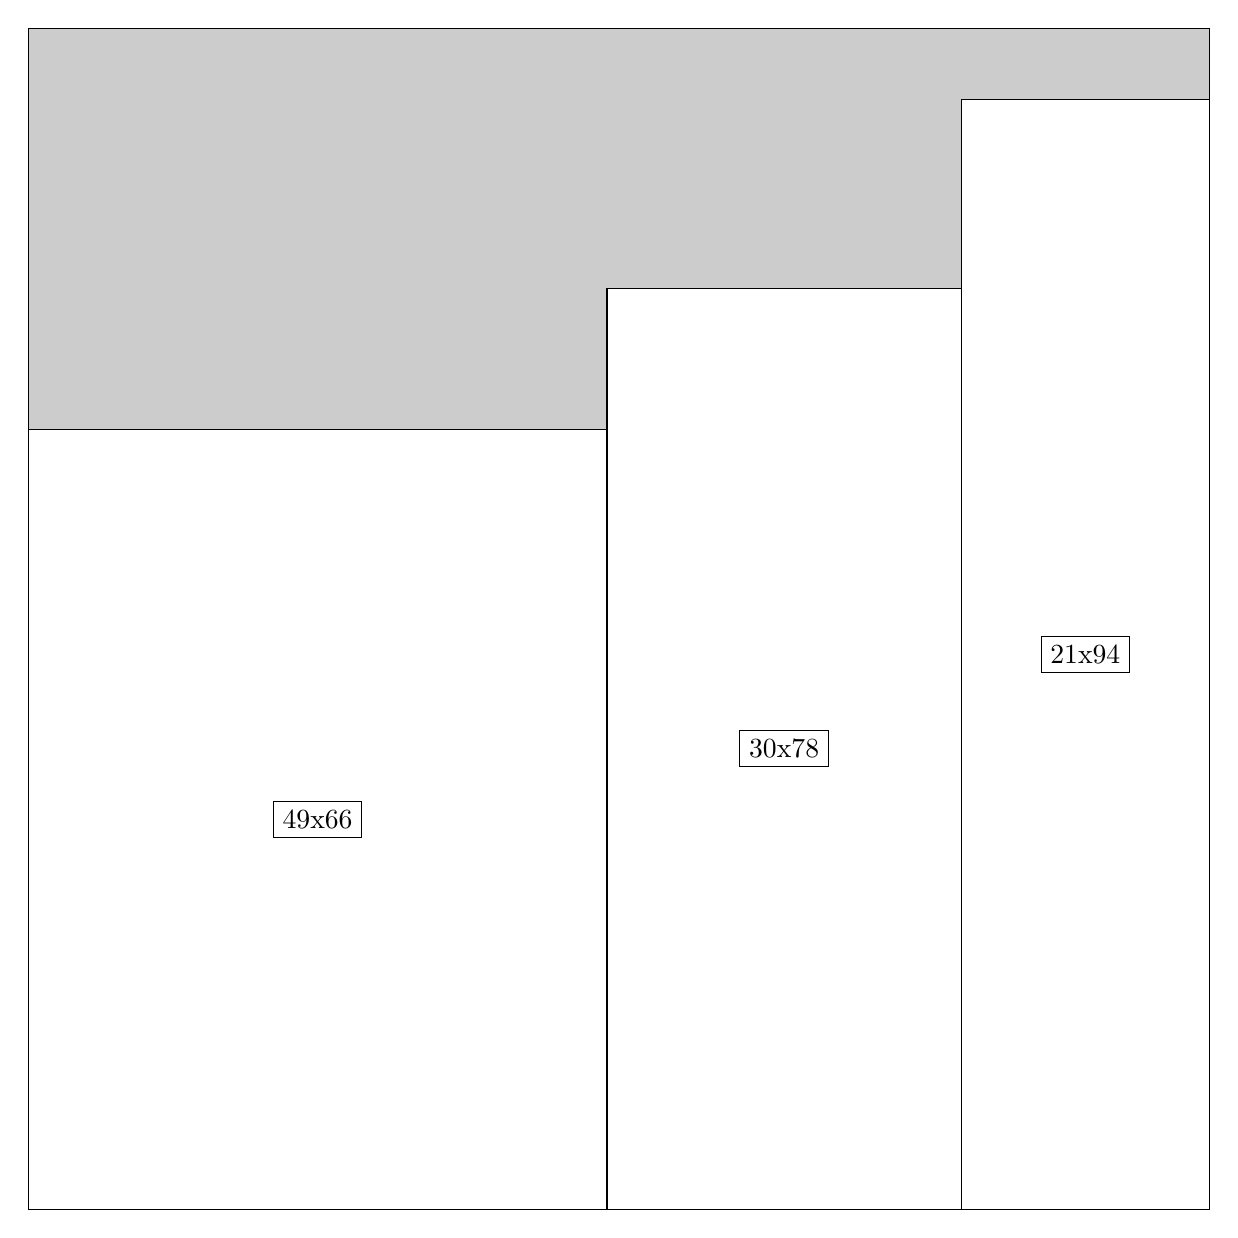
\begin{tikzpicture}[shorten >=1pt,scale=1.0,every node/.style={scale=1.0},->]
\tikzstyle{vertex}=[circle,fill=black!25,minimum size=14pt,inner sep=0pt]
\filldraw[fill=gray!40!white, draw=black] (0,0) rectangle (15.0,15.0);
\foreach \name/\x/\y/\w/\h in {21x94/11.85/0.0/3.15/14.1,30x78/7.35/0.0/4.5/11.7,49x66/0.0/0.0/7.35/9.9}
\filldraw[fill=white!40!white, draw=black] (\x,\y) rectangle node[draw] (\name) {\name} ++(\w,\h);
\end{tikzpicture}


w =21 , h =94 , x =79 , y =0 , v =1974
\par
w =30 , h =78 , x =49 , y =0 , v =2340
\par
w =49 , h =66 , x =0 , y =0 , v =3234
\par
\newpage


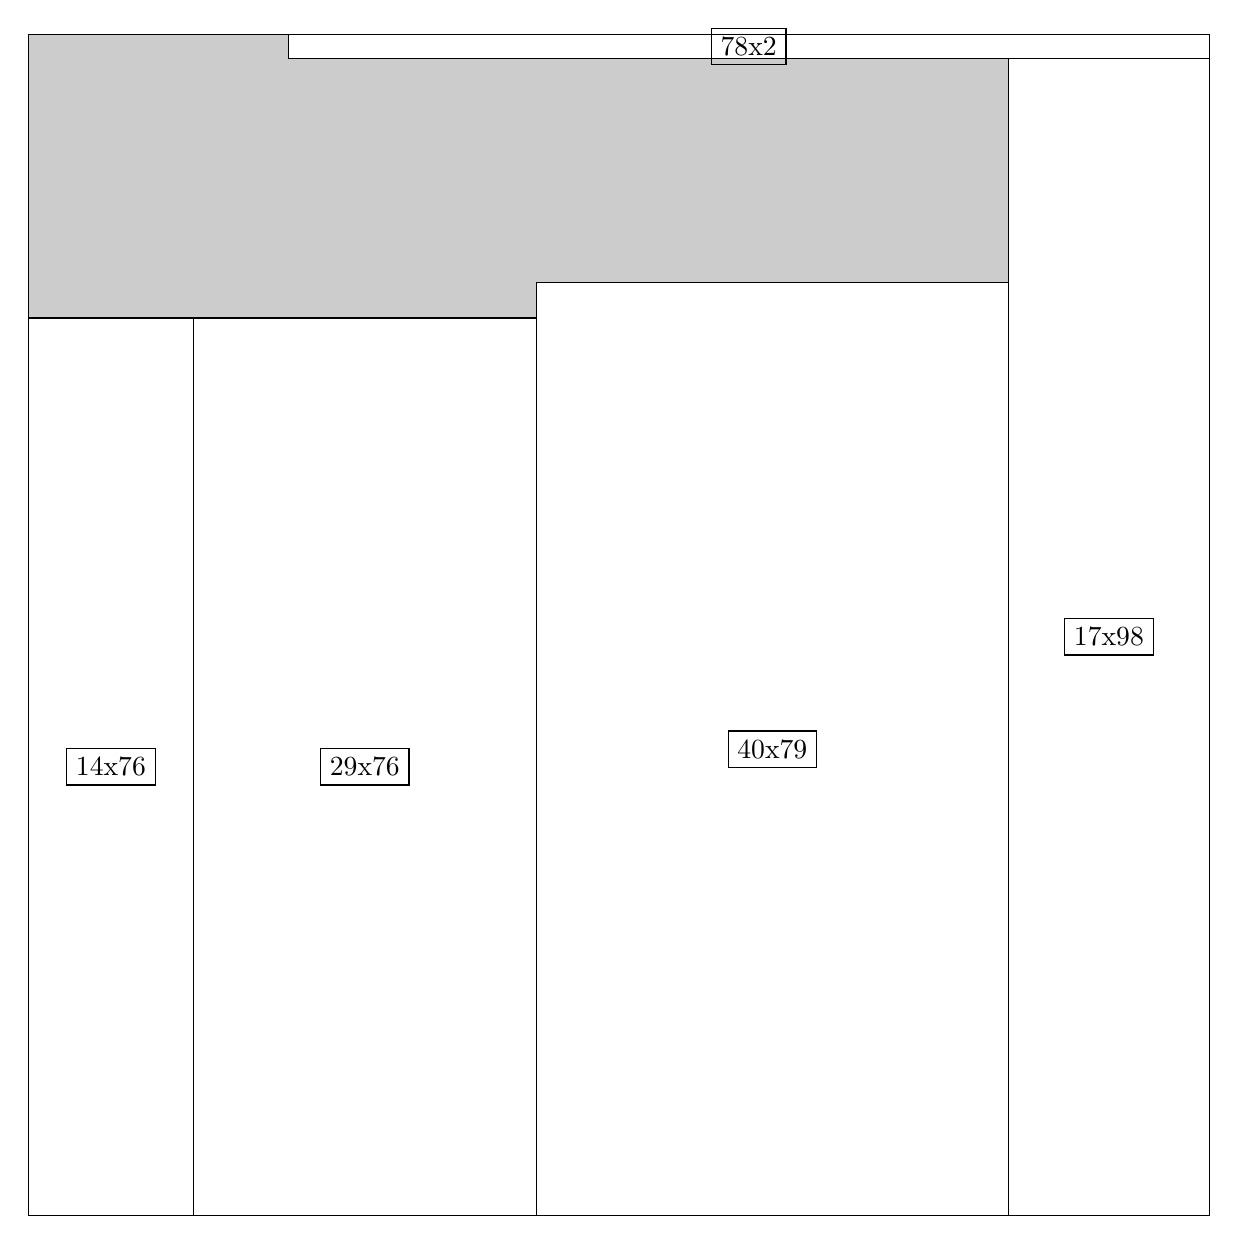
\begin{tikzpicture}[shorten >=1pt,scale=1.0,every node/.style={scale=1.0},->]
\tikzstyle{vertex}=[circle,fill=black!25,minimum size=14pt,inner sep=0pt]
\filldraw[fill=gray!40!white, draw=black] (0,0) rectangle (15.0,15.0);
\foreach \name/\x/\y/\w/\h in {17x98/12.45/0.0/2.55/14.7,40x79/6.45/0.0/6.0/11.85,29x76/2.1/0.0/4.35/11.4,14x76/0.0/0.0/2.1/11.4,78x2/3.3/14.7/11.7/0.3}
\filldraw[fill=white!40!white, draw=black] (\x,\y) rectangle node[draw] (\name) {\name} ++(\w,\h);
\end{tikzpicture}


w =17 , h =98 , x =83 , y =0 , v =1666
\par
w =40 , h =79 , x =43 , y =0 , v =3160
\par
w =29 , h =76 , x =14 , y =0 , v =2204
\par
w =14 , h =76 , x =0 , y =0 , v =1064
\par
w =78 , h =2 , x =22 , y =98 , v =156
\par
\newpage


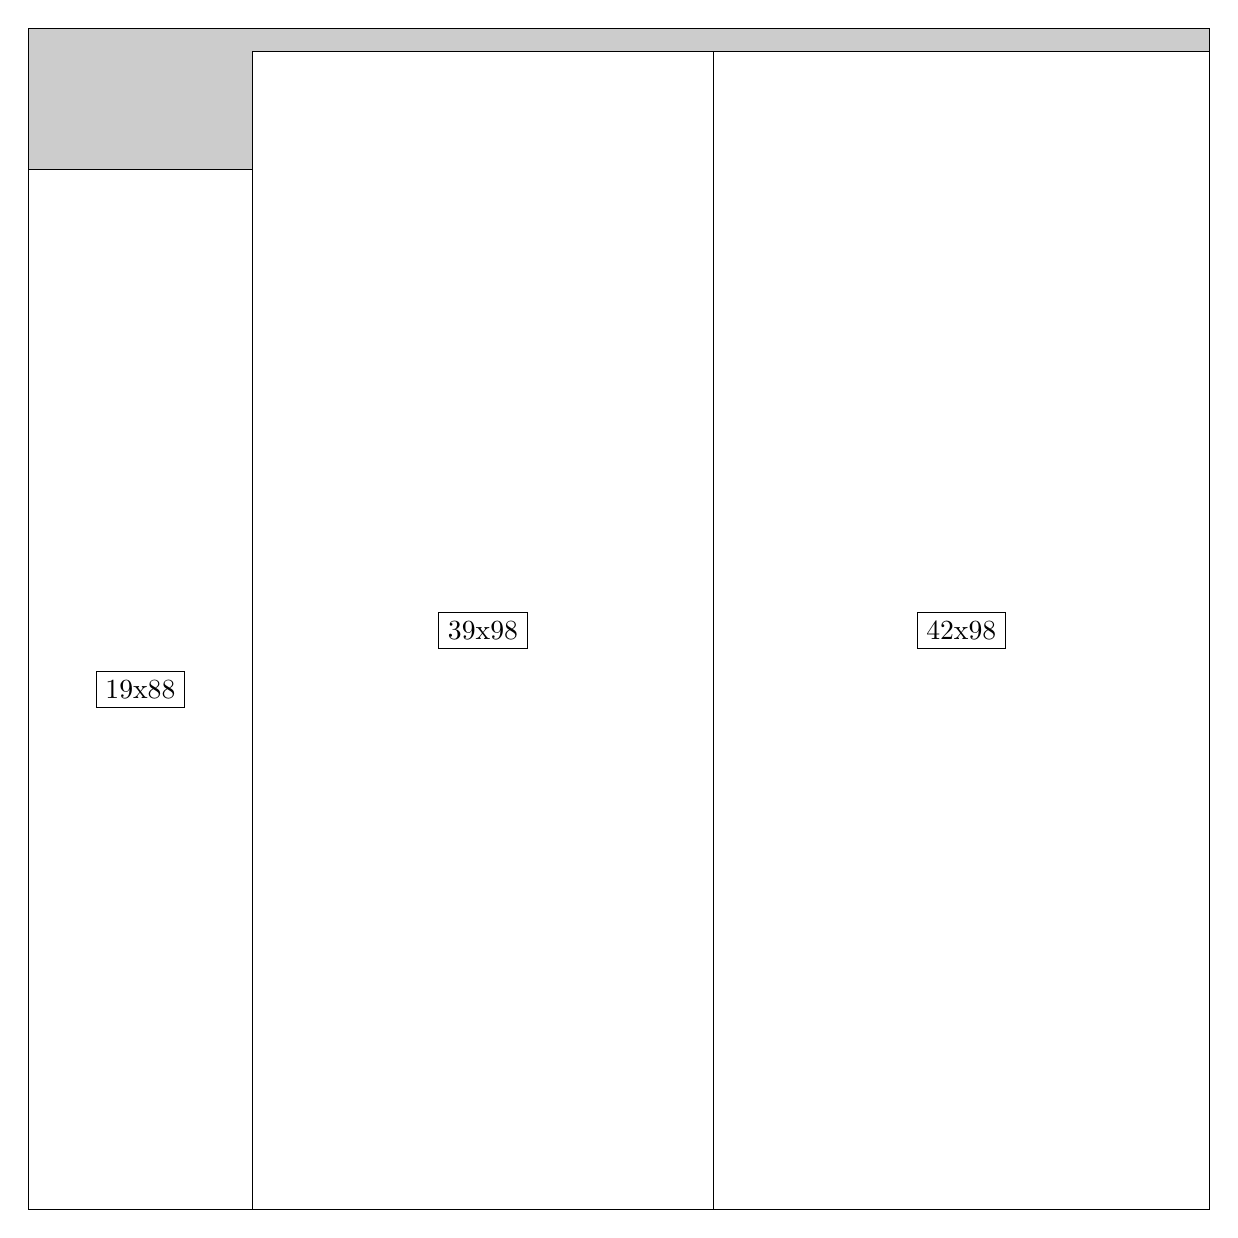
\begin{tikzpicture}[shorten >=1pt,scale=1.0,every node/.style={scale=1.0},->]
\tikzstyle{vertex}=[circle,fill=black!25,minimum size=14pt,inner sep=0pt]
\filldraw[fill=gray!40!white, draw=black] (0,0) rectangle (15.0,15.0);
\foreach \name/\x/\y/\w/\h in {42x98/8.7/0.0/6.3/14.7,39x98/2.85/0.0/5.85/14.7,19x88/0.0/0.0/2.85/13.2}
\filldraw[fill=white!40!white, draw=black] (\x,\y) rectangle node[draw] (\name) {\name} ++(\w,\h);
\end{tikzpicture}


w =42 , h =98 , x =58 , y =0 , v =4116
\par
w =39 , h =98 , x =19 , y =0 , v =3822
\par
w =19 , h =88 , x =0 , y =0 , v =1672
\par
\newpage


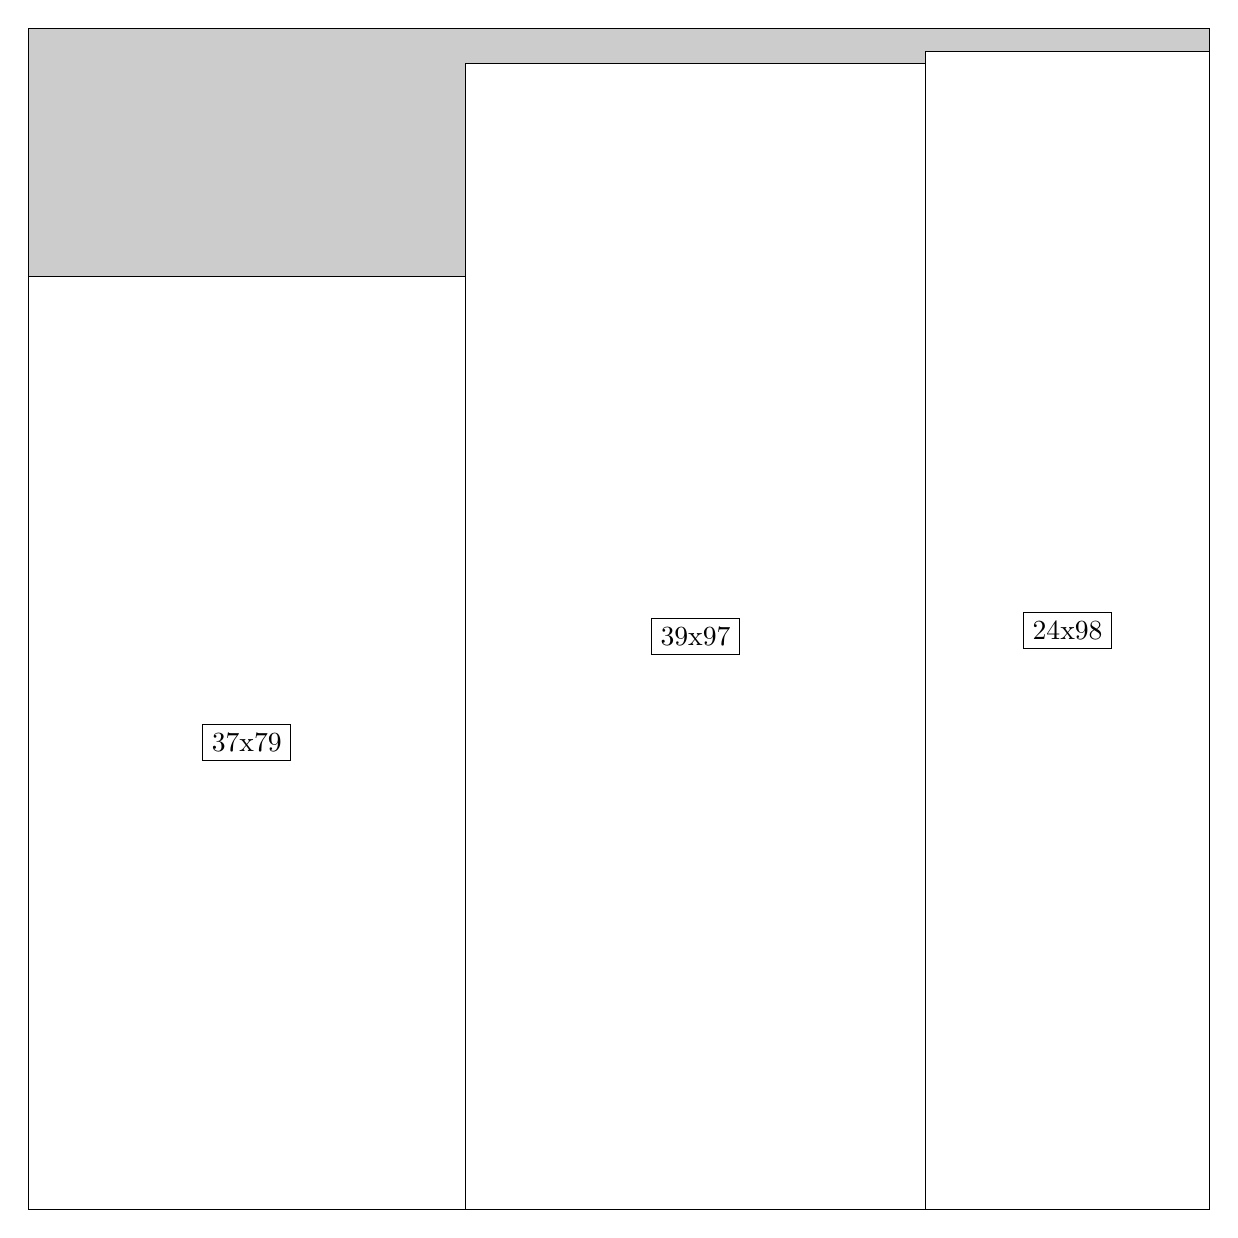
\begin{tikzpicture}[shorten >=1pt,scale=1.0,every node/.style={scale=1.0},->]
\tikzstyle{vertex}=[circle,fill=black!25,minimum size=14pt,inner sep=0pt]
\filldraw[fill=gray!40!white, draw=black] (0,0) rectangle (15.0,15.0);
\foreach \name/\x/\y/\w/\h in {24x98/11.4/0.0/3.5999999999999996/14.7,39x97/5.55/0.0/5.85/14.549999999999999,37x79/0.0/0.0/5.55/11.85}
\filldraw[fill=white!40!white, draw=black] (\x,\y) rectangle node[draw] (\name) {\name} ++(\w,\h);
\end{tikzpicture}


w =24 , h =98 , x =76 , y =0 , v =2352
\par
w =39 , h =97 , x =37 , y =0 , v =3783
\par
w =37 , h =79 , x =0 , y =0 , v =2923
\par
\newpage


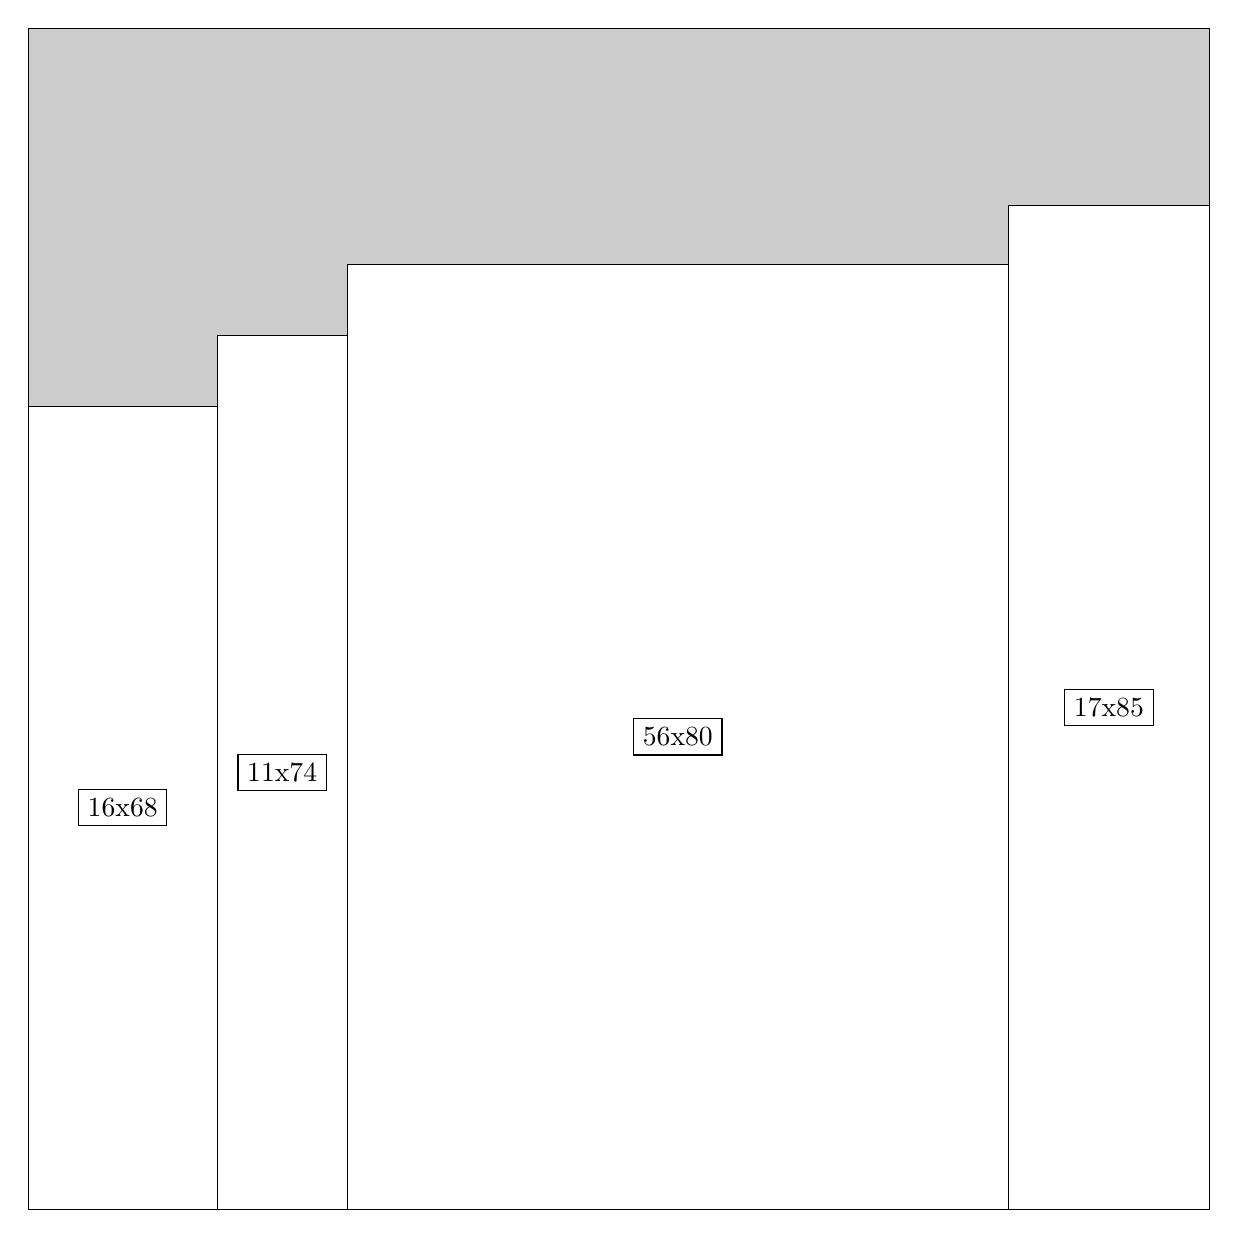
\begin{tikzpicture}[shorten >=1pt,scale=1.0,every node/.style={scale=1.0},->]
\tikzstyle{vertex}=[circle,fill=black!25,minimum size=14pt,inner sep=0pt]
\filldraw[fill=gray!40!white, draw=black] (0,0) rectangle (15.0,15.0);
\foreach \name/\x/\y/\w/\h in {17x85/12.45/0.0/2.55/12.75,56x80/4.05/0.0/8.4/12.0,11x74/2.4/0.0/1.65/11.1,16x68/0.0/0.0/2.4/10.2}
\filldraw[fill=white!40!white, draw=black] (\x,\y) rectangle node[draw] (\name) {\name} ++(\w,\h);
\end{tikzpicture}


w =17 , h =85 , x =83 , y =0 , v =1445
\par
w =56 , h =80 , x =27 , y =0 , v =4480
\par
w =11 , h =74 , x =16 , y =0 , v =814
\par
w =16 , h =68 , x =0 , y =0 , v =1088
\par
\newpage


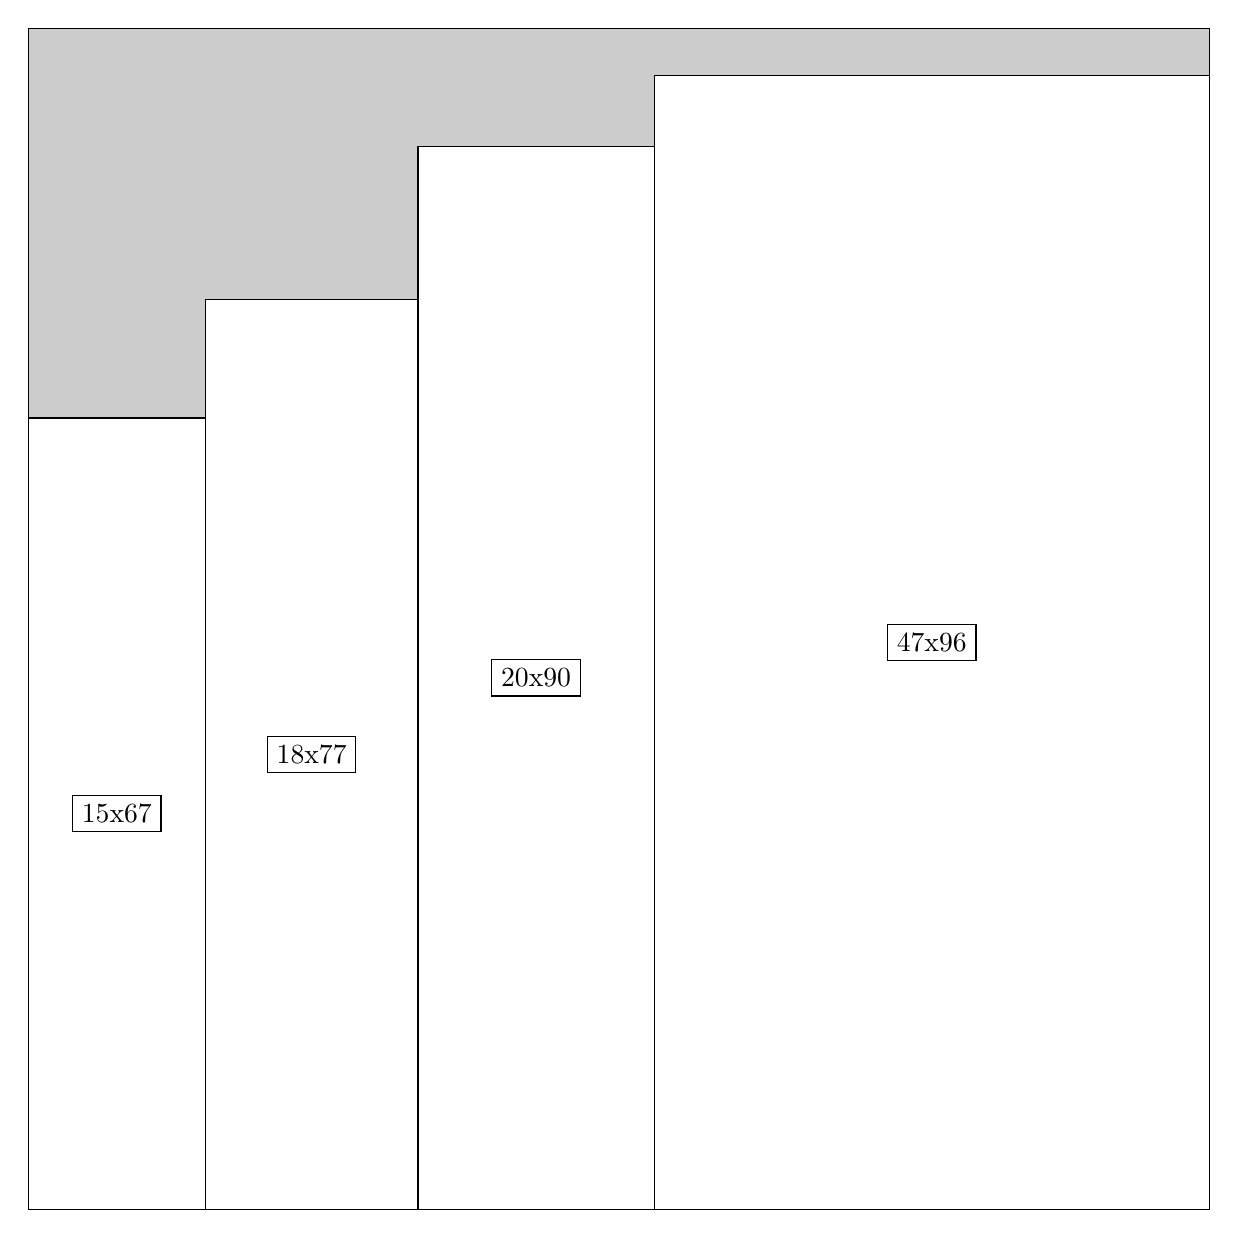
\begin{tikzpicture}[shorten >=1pt,scale=1.0,every node/.style={scale=1.0},->]
\tikzstyle{vertex}=[circle,fill=black!25,minimum size=14pt,inner sep=0pt]
\filldraw[fill=gray!40!white, draw=black] (0,0) rectangle (15.0,15.0);
\foreach \name/\x/\y/\w/\h in {47x96/7.949999999999999/0.0/7.05/14.399999999999999,20x90/4.95/0.0/3.0/13.5,18x77/2.25/0.0/2.6999999999999997/11.549999999999999,15x67/0.0/0.0/2.25/10.049999999999999}
\filldraw[fill=white!40!white, draw=black] (\x,\y) rectangle node[draw] (\name) {\name} ++(\w,\h);
\end{tikzpicture}


w =47 , h =96 , x =53 , y =0 , v =4512
\par
w =20 , h =90 , x =33 , y =0 , v =1800
\par
w =18 , h =77 , x =15 , y =0 , v =1386
\par
w =15 , h =67 , x =0 , y =0 , v =1005
\par
\newpage


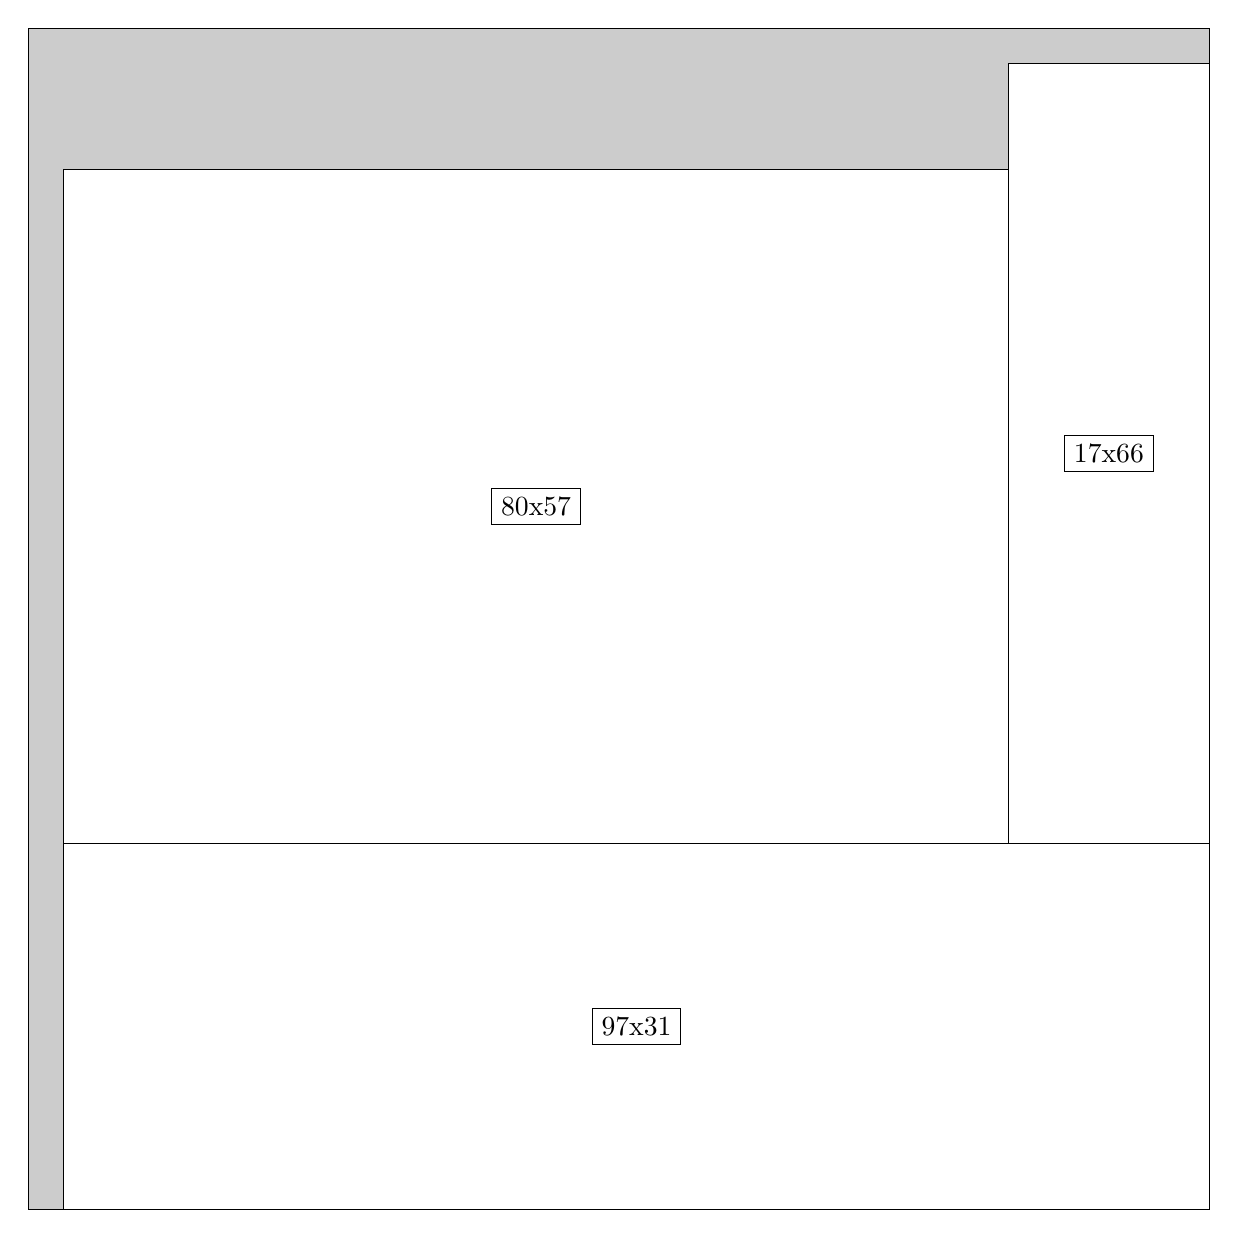
\begin{tikzpicture}[shorten >=1pt,scale=1.0,every node/.style={scale=1.0},->]
\tikzstyle{vertex}=[circle,fill=black!25,minimum size=14pt,inner sep=0pt]
\filldraw[fill=gray!40!white, draw=black] (0,0) rectangle (15.0,15.0);
\foreach \name/\x/\y/\w/\h in {97x31/0.44999999999999996/0.0/14.549999999999999/4.6499999999999995,17x66/12.45/4.6499999999999995/2.55/9.9,80x57/0.44999999999999996/4.6499999999999995/12.0/8.549999999999999}
\filldraw[fill=white!40!white, draw=black] (\x,\y) rectangle node[draw] (\name) {\name} ++(\w,\h);
\end{tikzpicture}


w =97 , h =31 , x =3 , y =0 , v =3007
\par
w =17 , h =66 , x =83 , y =31 , v =1122
\par
w =80 , h =57 , x =3 , y =31 , v =4560
\par
\newpage


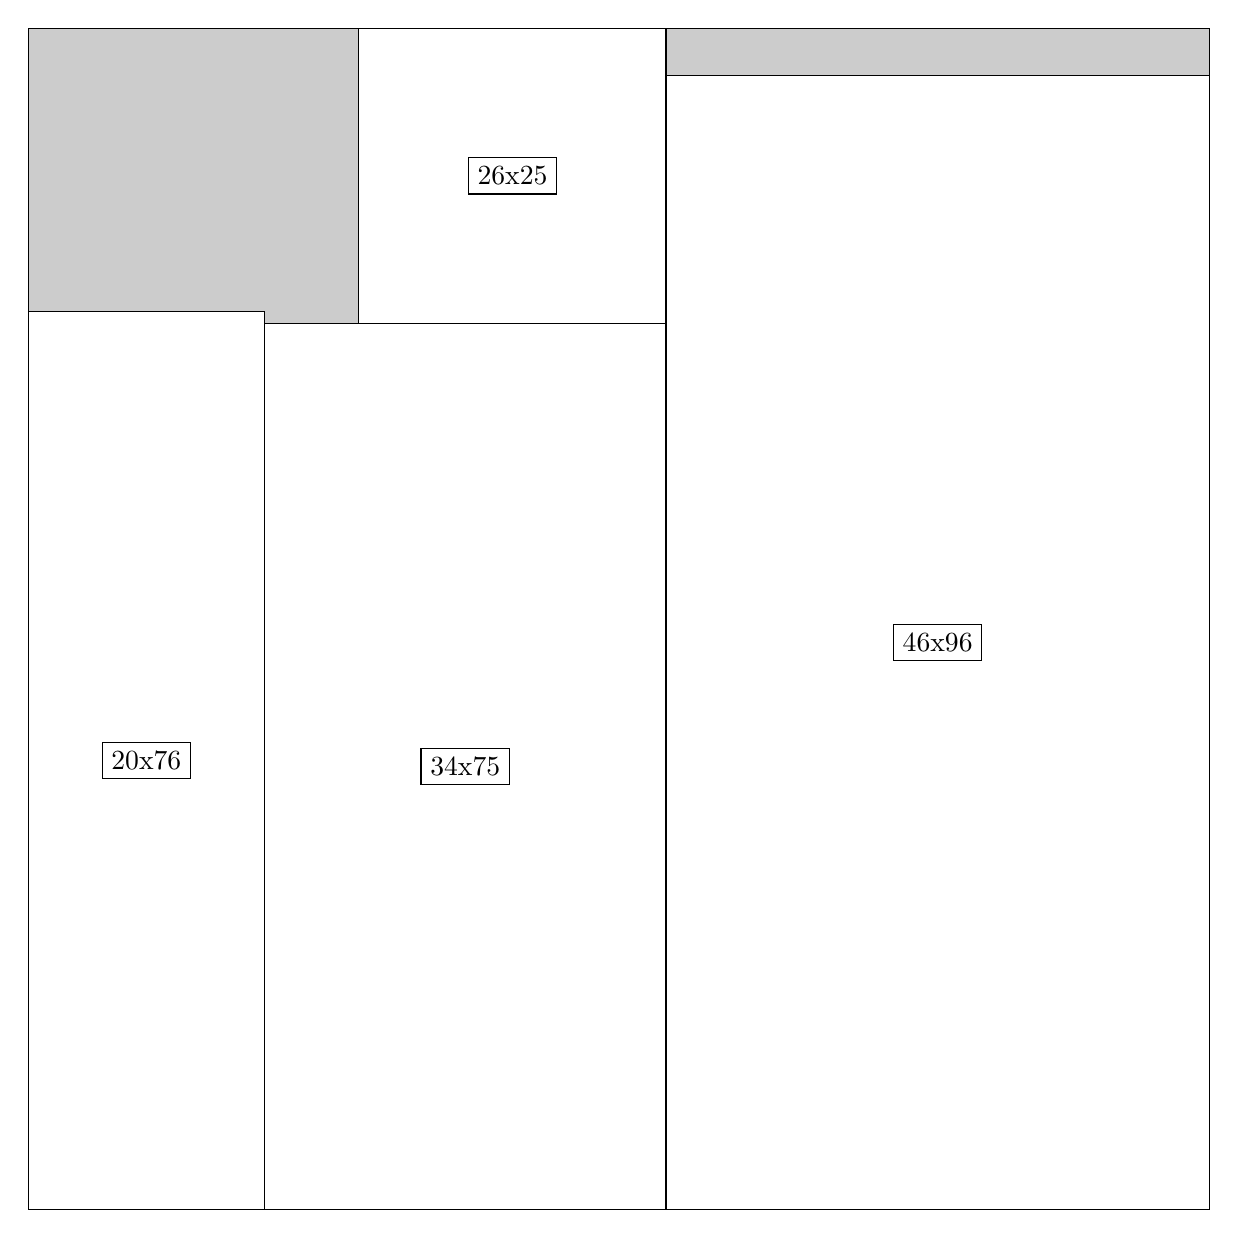
\begin{tikzpicture}[shorten >=1pt,scale=1.0,every node/.style={scale=1.0},->]
\tikzstyle{vertex}=[circle,fill=black!25,minimum size=14pt,inner sep=0pt]
\filldraw[fill=gray!40!white, draw=black] (0,0) rectangle (15.0,15.0);
\foreach \name/\x/\y/\w/\h in {46x96/8.1/0.0/6.8999999999999995/14.399999999999999,34x75/3.0/0.0/5.1/11.25,26x25/4.2/11.25/3.9/3.75,20x76/0.0/0.0/3.0/11.4}
\filldraw[fill=white!40!white, draw=black] (\x,\y) rectangle node[draw] (\name) {\name} ++(\w,\h);
\end{tikzpicture}


w =46 , h =96 , x =54 , y =0 , v =4416
\par
w =34 , h =75 , x =20 , y =0 , v =2550
\par
w =26 , h =25 , x =28 , y =75 , v =650
\par
w =20 , h =76 , x =0 , y =0 , v =1520
\par
\newpage


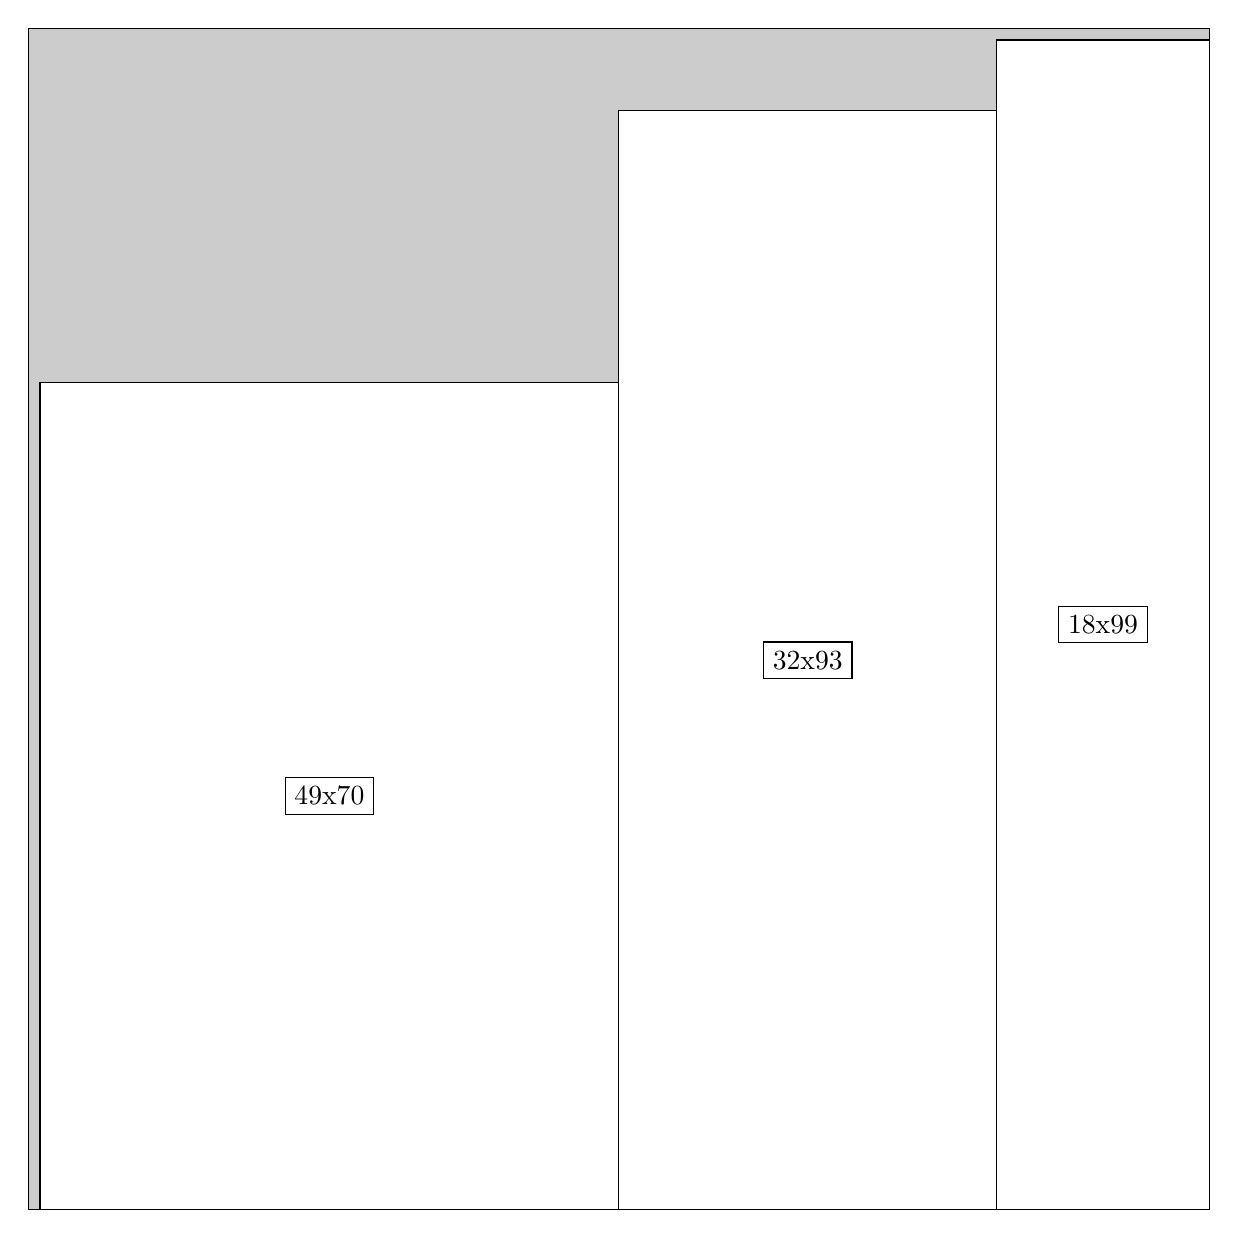
\begin{tikzpicture}[shorten >=1pt,scale=1.0,every node/.style={scale=1.0},->]
\tikzstyle{vertex}=[circle,fill=black!25,minimum size=14pt,inner sep=0pt]
\filldraw[fill=gray!40!white, draw=black] (0,0) rectangle (15.0,15.0);
\foreach \name/\x/\y/\w/\h in {18x99/12.299999999999999/0.0/2.6999999999999997/14.85,32x93/7.5/0.0/4.8/13.95,49x70/0.15/0.0/7.35/10.5}
\filldraw[fill=white!40!white, draw=black] (\x,\y) rectangle node[draw] (\name) {\name} ++(\w,\h);
\end{tikzpicture}


w =18 , h =99 , x =82 , y =0 , v =1782
\par
w =32 , h =93 , x =50 , y =0 , v =2976
\par
w =49 , h =70 , x =1 , y =0 , v =3430
\par
\newpage


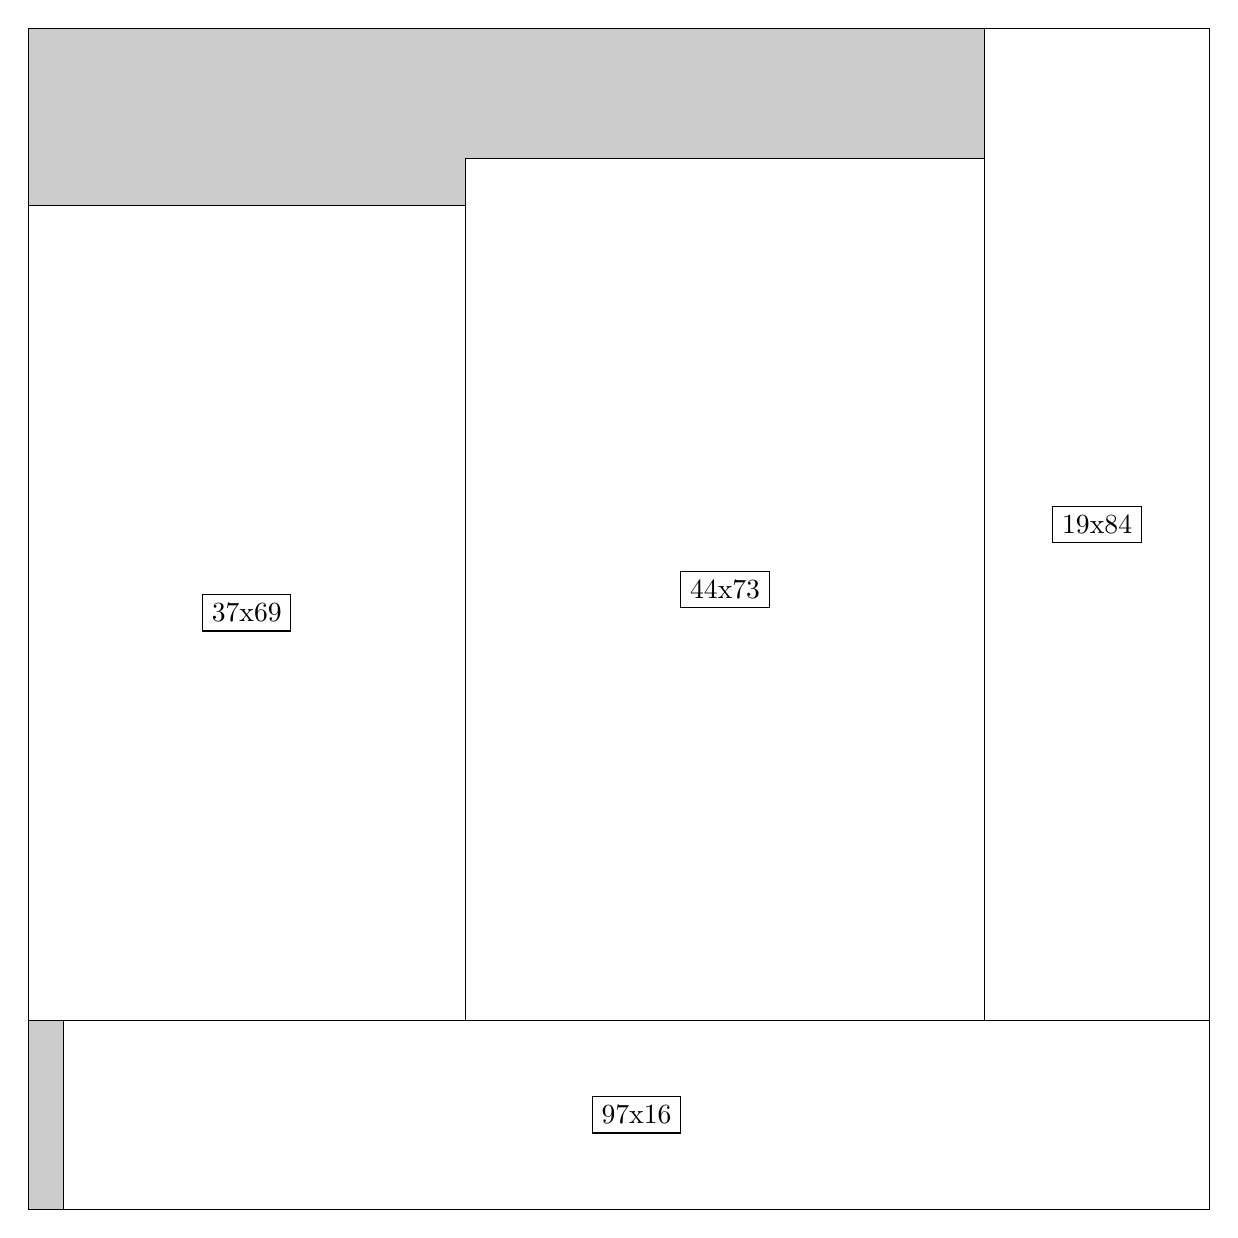
\begin{tikzpicture}[shorten >=1pt,scale=1.0,every node/.style={scale=1.0},->]
\tikzstyle{vertex}=[circle,fill=black!25,minimum size=14pt,inner sep=0pt]
\filldraw[fill=gray!40!white, draw=black] (0,0) rectangle (15.0,15.0);
\foreach \name/\x/\y/\w/\h in {97x16/0.44999999999999996/0.0/14.549999999999999/2.4,19x84/12.15/2.4/2.85/12.6,44x73/5.55/2.4/6.6/10.95,37x69/0.0/2.4/5.55/10.35}
\filldraw[fill=white!40!white, draw=black] (\x,\y) rectangle node[draw] (\name) {\name} ++(\w,\h);
\end{tikzpicture}


w =97 , h =16 , x =3 , y =0 , v =1552
\par
w =19 , h =84 , x =81 , y =16 , v =1596
\par
w =44 , h =73 , x =37 , y =16 , v =3212
\par
w =37 , h =69 , x =0 , y =16 , v =2553
\par
\newpage


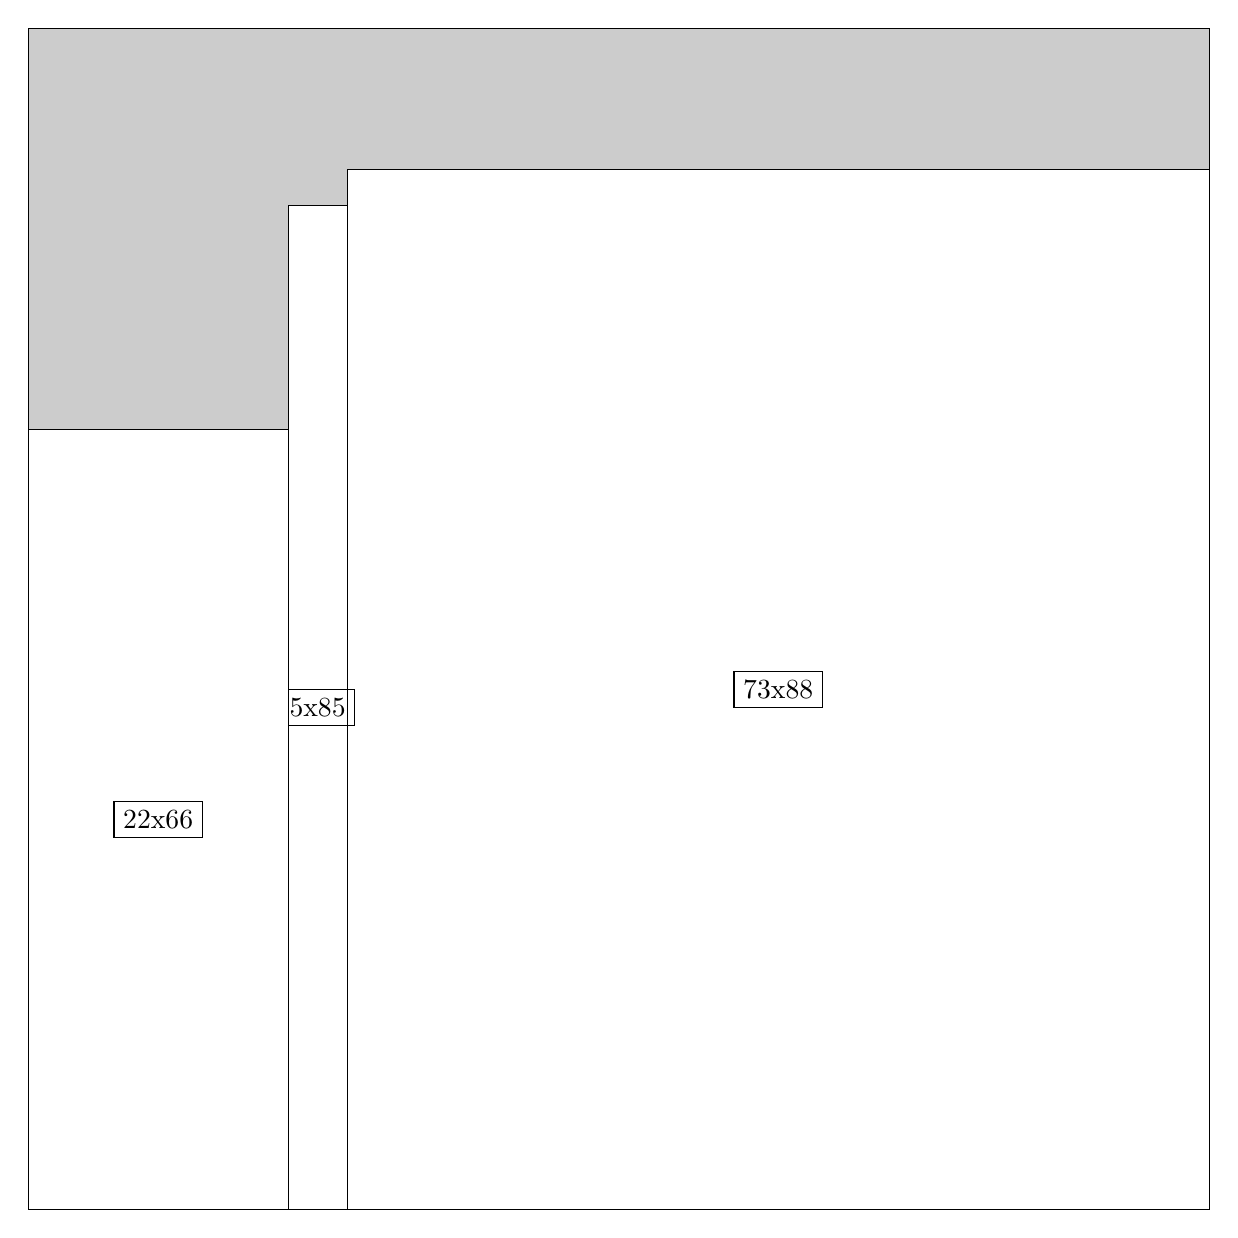
\begin{tikzpicture}[shorten >=1pt,scale=1.0,every node/.style={scale=1.0},->]
\tikzstyle{vertex}=[circle,fill=black!25,minimum size=14pt,inner sep=0pt]
\filldraw[fill=gray!40!white, draw=black] (0,0) rectangle (15.0,15.0);
\foreach \name/\x/\y/\w/\h in {73x88/4.05/0.0/10.95/13.2,5x85/3.3/0.0/0.75/12.75,22x66/0.0/0.0/3.3/9.9}
\filldraw[fill=white!40!white, draw=black] (\x,\y) rectangle node[draw] (\name) {\name} ++(\w,\h);
\end{tikzpicture}


w =73 , h =88 , x =27 , y =0 , v =6424
\par
w =5 , h =85 , x =22 , y =0 , v =425
\par
w =22 , h =66 , x =0 , y =0 , v =1452
\par
\newpage


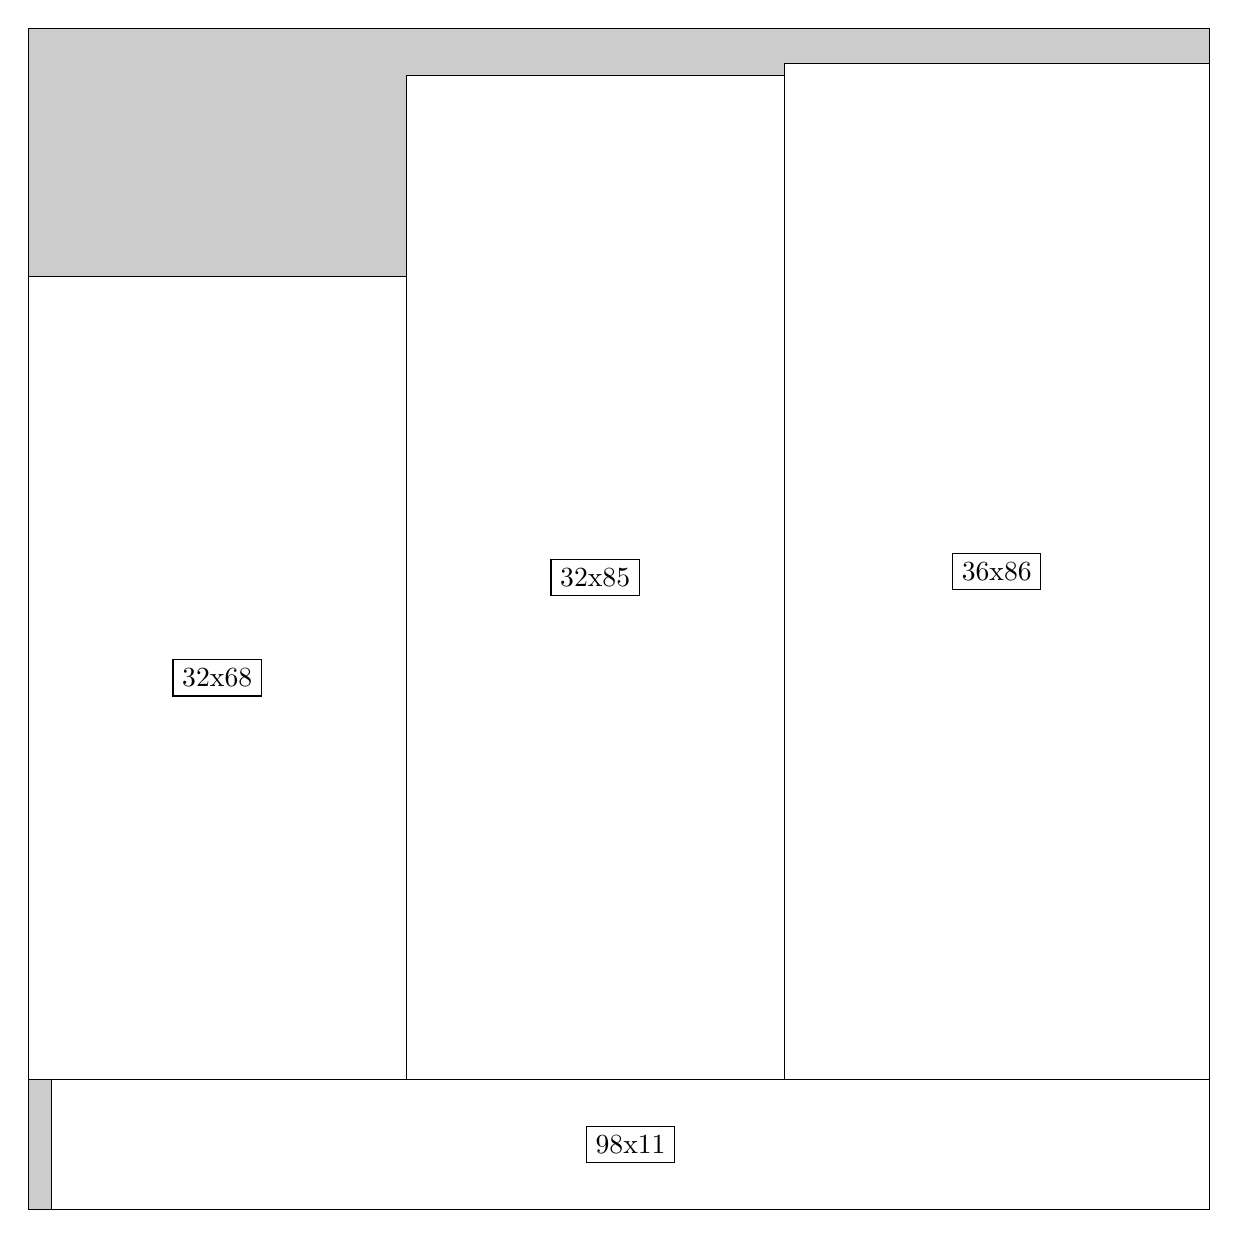
\begin{tikzpicture}[shorten >=1pt,scale=1.0,every node/.style={scale=1.0},->]
\tikzstyle{vertex}=[circle,fill=black!25,minimum size=14pt,inner sep=0pt]
\filldraw[fill=gray!40!white, draw=black] (0,0) rectangle (15.0,15.0);
\foreach \name/\x/\y/\w/\h in {98x11/0.3/0.0/14.7/1.65,36x86/9.6/1.65/5.3999999999999995/12.9,32x85/4.8/1.65/4.8/12.75,32x68/0.0/1.65/4.8/10.2}
\filldraw[fill=white!40!white, draw=black] (\x,\y) rectangle node[draw] (\name) {\name} ++(\w,\h);
\end{tikzpicture}


w =98 , h =11 , x =2 , y =0 , v =1078
\par
w =36 , h =86 , x =64 , y =11 , v =3096
\par
w =32 , h =85 , x =32 , y =11 , v =2720
\par
w =32 , h =68 , x =0 , y =11 , v =2176
\par
\newpage


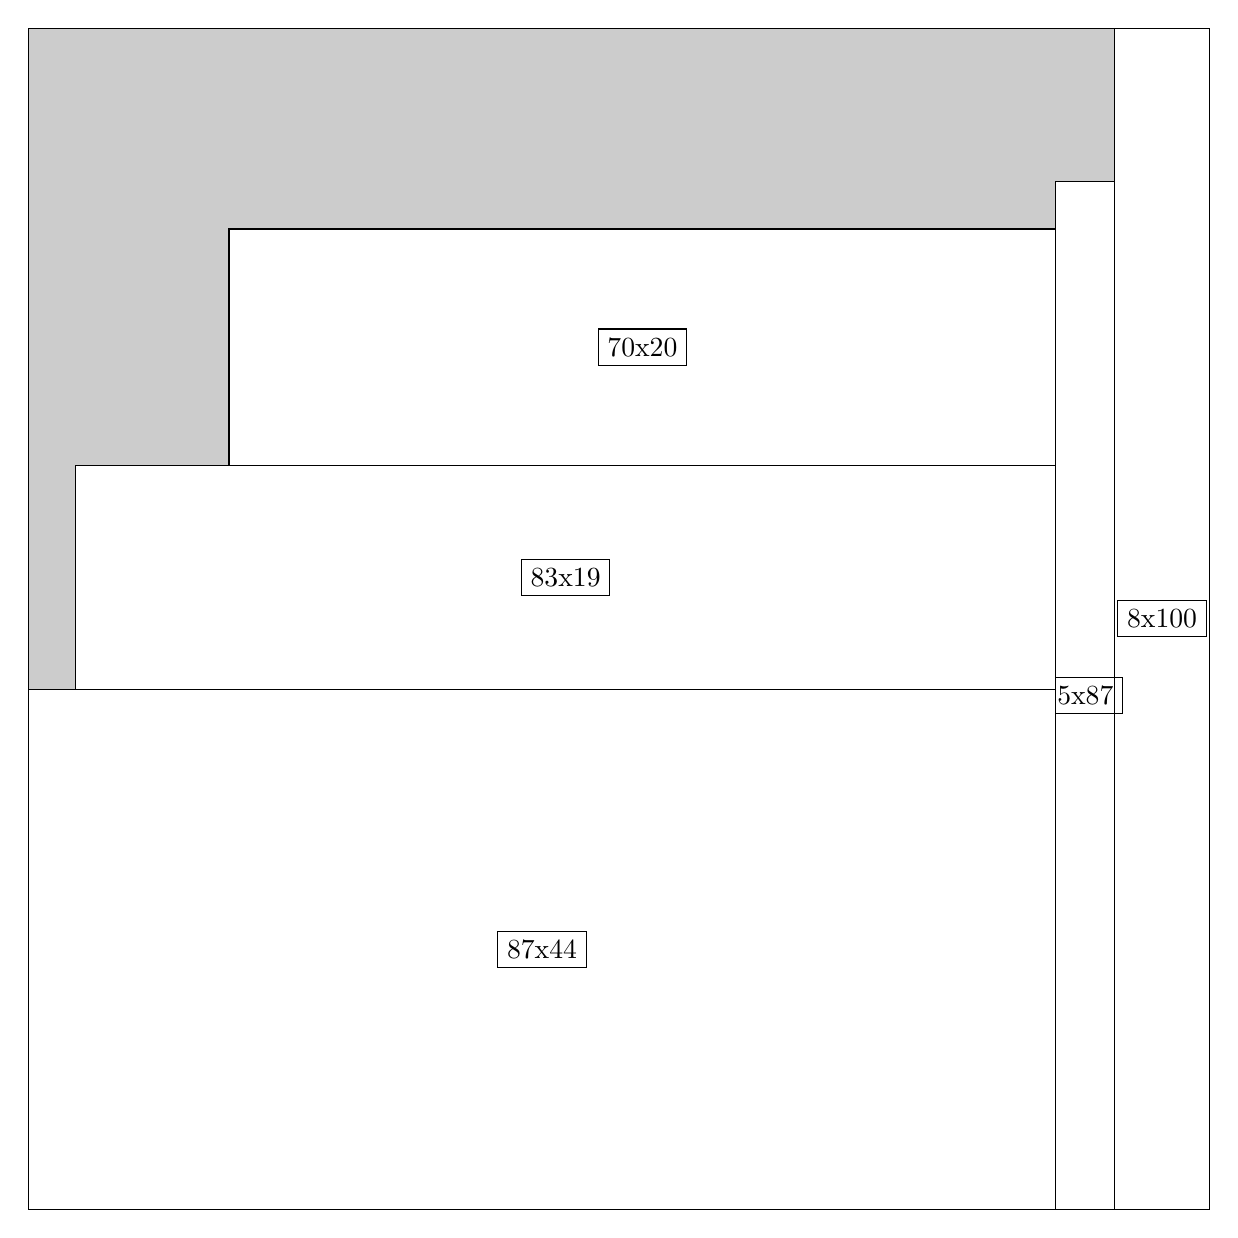
\begin{tikzpicture}[shorten >=1pt,scale=1.0,every node/.style={scale=1.0},->]
\tikzstyle{vertex}=[circle,fill=black!25,minimum size=14pt,inner sep=0pt]
\filldraw[fill=gray!40!white, draw=black] (0,0) rectangle (15.0,15.0);
\foreach \name/\x/\y/\w/\h in {8x100/13.799999999999999/0.0/1.2/15.0,5x87/13.049999999999999/0.0/0.75/13.049999999999999,87x44/0.0/0.0/13.049999999999999/6.6,83x19/0.6/6.6/12.45/2.85,70x20/2.55/9.45/10.5/3.0}
\filldraw[fill=white!40!white, draw=black] (\x,\y) rectangle node[draw] (\name) {\name} ++(\w,\h);
\end{tikzpicture}


w =8 , h =100 , x =92 , y =0 , v =800
\par
w =5 , h =87 , x =87 , y =0 , v =435
\par
w =87 , h =44 , x =0 , y =0 , v =3828
\par
w =83 , h =19 , x =4 , y =44 , v =1577
\par
w =70 , h =20 , x =17 , y =63 , v =1400
\par
\newpage


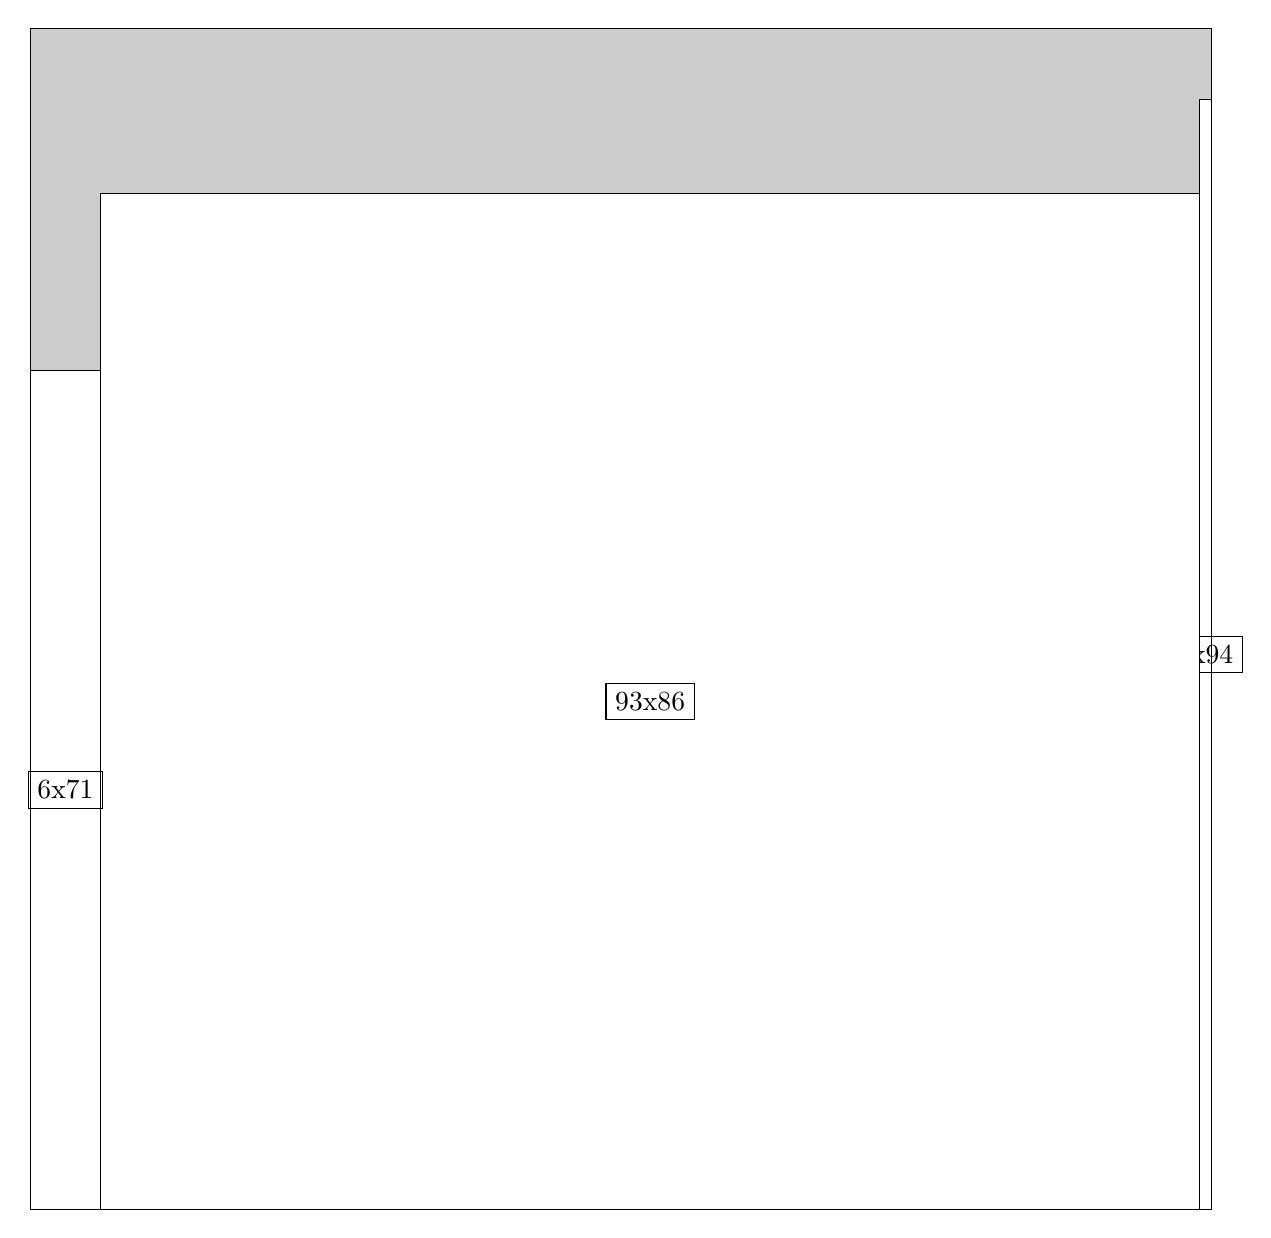
\begin{tikzpicture}[shorten >=1pt,scale=1.0,every node/.style={scale=1.0},->]
\tikzstyle{vertex}=[circle,fill=black!25,minimum size=14pt,inner sep=0pt]
\filldraw[fill=gray!40!white, draw=black] (0,0) rectangle (15.0,15.0);
\foreach \name/\x/\y/\w/\h in {1x94/14.85/0.0/0.15/14.1,93x86/0.8999999999999999/0.0/13.95/12.9,6x71/0.0/0.0/0.8999999999999999/10.65}
\filldraw[fill=white!40!white, draw=black] (\x,\y) rectangle node[draw] (\name) {\name} ++(\w,\h);
\end{tikzpicture}


w =1 , h =94 , x =99 , y =0 , v =94
\par
w =93 , h =86 , x =6 , y =0 , v =7998
\par
w =6 , h =71 , x =0 , y =0 , v =426
\par
\newpage


\end{document}